\chapter{Implementation analysis}
%co delam a jak to delam
The practical part of this work is focused on these tasks:
\begin{itemize}
\item POS tagging \\
\textit{input}: a word \\
\textit{output}: part-of-speech tags -- as noun, pronoun, punctuation mark etc.
\item lemmatization \\
\textit{input:} a word \\
\textit{output:} lemma -- a base form of a given words, meaning for example nominative of singular for nouns or infinitive for verbs. 
\item sentiment analysis \\
\textit{input:} a sentence or a sequence of sentences \\
\textit{output:} prevailing sentiment of the input from categories: neutral, positive, negative.
\todo{doplnit diskuzi o ruzných možnostech definice}
\end{itemize}.
\label{chap:impl}
This chapter describes implemented linguistic models. As mentioned before, this work implements models for three Czech NLP tasks: tagging, lemmatization and sentiment analysis. Common model for first two tasks develops on the paper by \cite[]{straka2019czech} focused on application of contextual embeddings produced by language models as Bert %todo cite
 or Flair. %todo cite. 
 Third task, sentiment analysis, is perfomed by adding only one fully-connected layer at the top of bert model. So in the opposite to previous tasks, no sophisticated handcrafted pipeline is built and model relies only on the network powers of language structure representation.
 \section{POS tagging and lemmatization model}
The model for this part is build upon a model (and a code) for previous work on Czech NLP processing with contextual embeddings \cite[]{straka2019czech}. Data preparation %todo trida s odkazem do github
pipeline - tokenization and sentence segmentation is taken over from the paper as well as base structure of lemmatizer and tagger network. 


\subsection{Dataset and preprocessing}
Dataset for these tasks is based on Prague Dependency Treebank (PDT), specifically version 3.5, which is PDT edition from year 2018. Dataset is divided into three parts - train, dtest and etest. Second one is used as development set while the third one as a test set for validation. %todo citace %jak vypadaji vstupni data - ukazka z tech dat co mam primo!!!
Data consists of sentences with lemmas and tags.Input sentences are preprocessed as follows:
\begin{itemize}
\item white space deletion
\item mapping characters -- all unknown dev and test characters are then mapped into one \textit{unk} token. 
\item mapping  words from train into integers -- all unknown dev and test words are then mapped into one \textit{unk} token. 
\end{itemize}


%jak vypadají vstupní data?

%jaky je preprocessing dat
	%odebrani mezer (rstrip)
	%co je analyses?
	%co je lemma rule
	%mapovani pismen jen ta co byla v train, jinak unk, totez slova
	%tedy parsování na slova a věty
	%bertí embeddingy
		%precomputed
		%bert segments ... ke ktere vete a slovu segmenty patri
		%bert subwords .. subwordy - proc subwordy a ze jsou v kontextu a proto musim s vetou celou!!
		%udelat z toho tensor
		
\subsection{Network}
Lemmatization as well as tagging are considered to be classification tasks (same as in \cite[]{straka2019czech}), i.e. lemmatization classification target are lemma generating rules and tagging target is tag, of course. Both tasks share one network.

Script allows training of these model variants:
\begin{itemize}
\item baseline model -- original implementation %todo zdroj
of network as described in figure %todo obrazek a zdroj co to dela
\\ \textbf{Embeddings:} %TODO popsat poradne tvar
Model contains potentially embeddings of four types -- pretrained word2vec embeddings %todo zdroj
, word embeddings trained with network, bert embeddings (just in some models as described later) and character-level embeddings.
\item label smoothing -- baseline model with label smoothing %todo zdroj na label smoothing a zdroj na vysvetleni v nektere casti
\item bert embeddings -- model can take precomputed bert embeddings as an input, otherwise embeddings are computed at the beginning and also saved for further use. In this case, data are tokenized by BERT tokenizer. Same principle is used for unknown words as before. Embeddings for word segments are averaged for each original input word, as BERT word segments and sentence words does not correspond to each other one to one. These embeddings serves as additional input to the network as in figure %TODO  %TODO see sectionBert embeddings are contextualized %see section so whole sentence is input into BERT tokenizer.
\item BERT finetunning -- In contrast to the BERT embeddings model, in this case BERT embeddings are also trained during network training, i.e. whole BERT network is chained to baseline network instead of embedding numbers only, gradients are backpropagated throw whole new network and weights are updated also in the BERT part of network.
\end{itemize}
All classification can be done with or without use of a morphological dictionary MorFlex %todo reference
. If the option with dictionary is used, generated tags and lemmas are chosen just from the dictionary. So it is selected lemma and/or tag with maximal likelihood, but just from those presented in the dictionary.

\centering
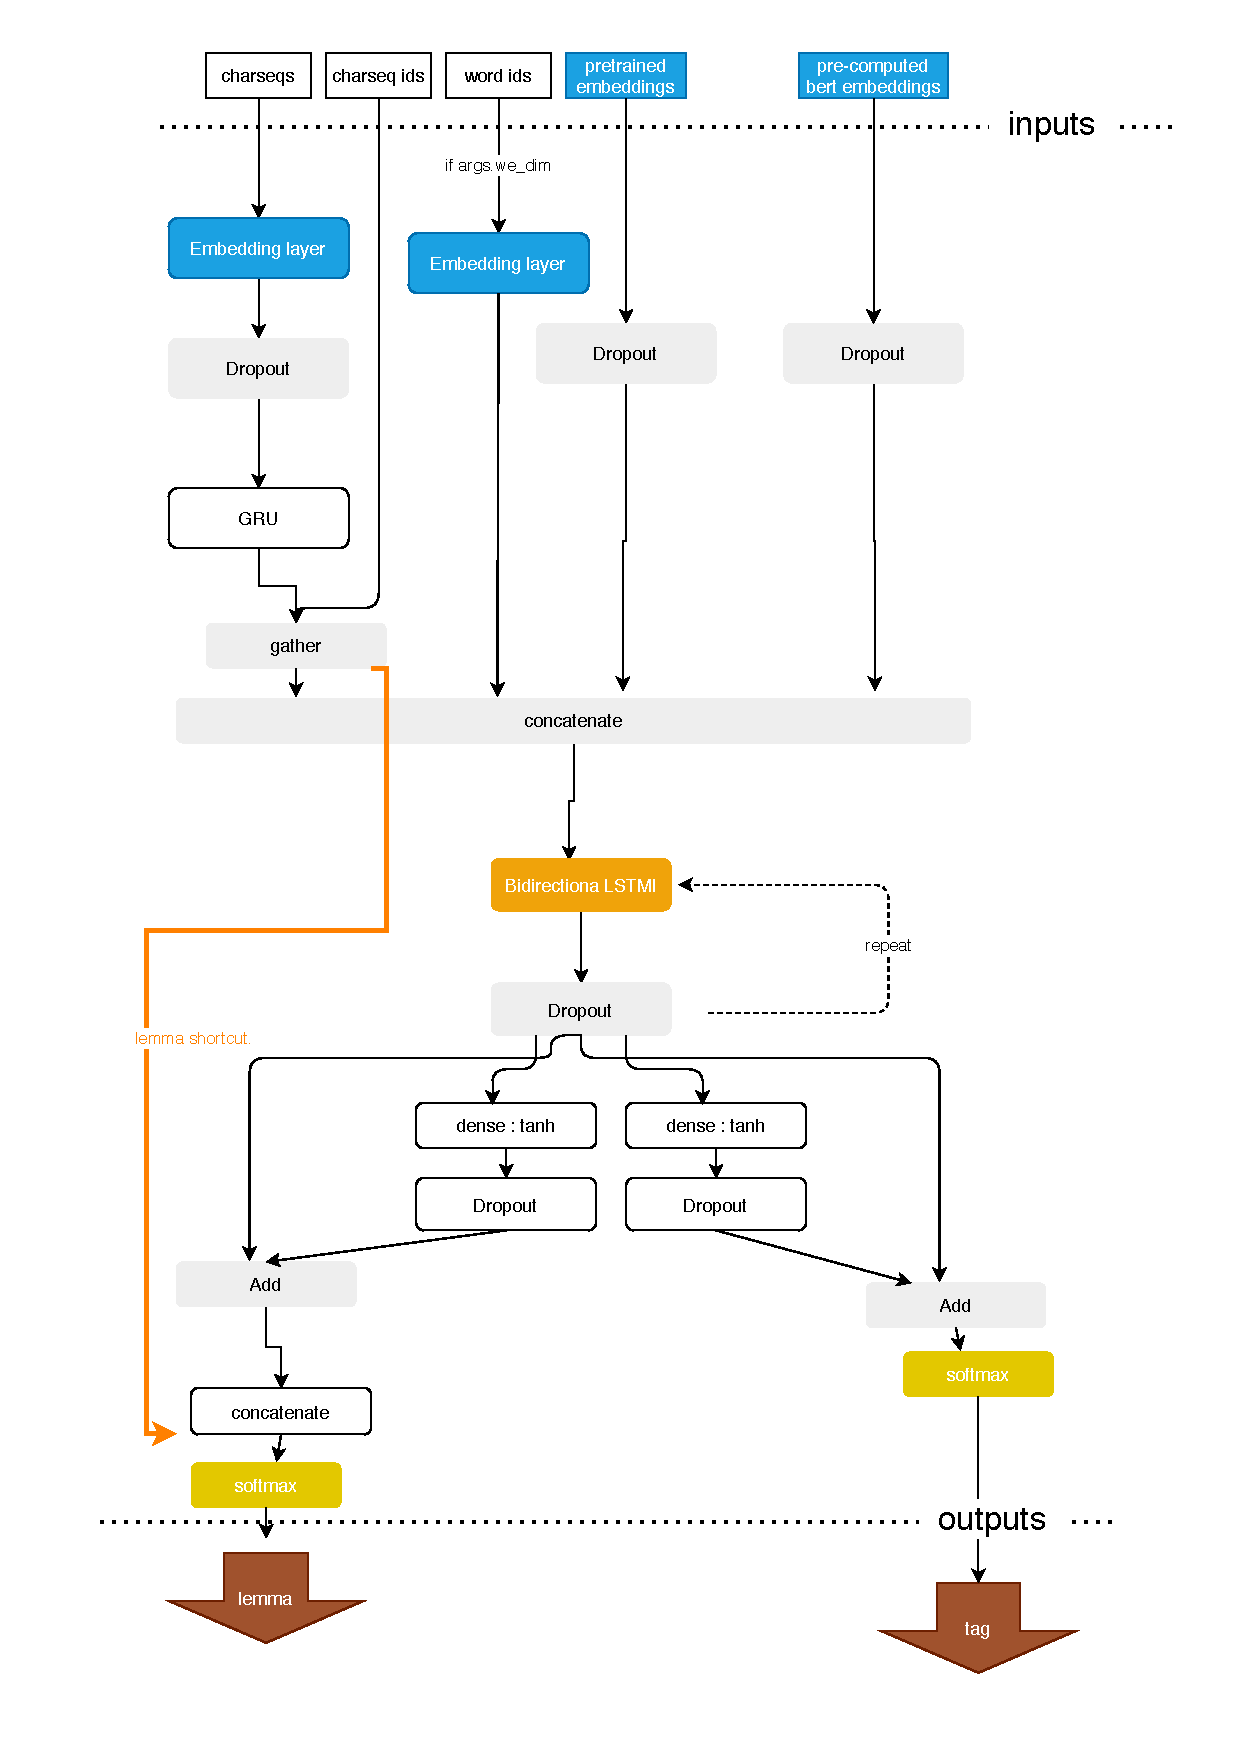
\includegraphics[width=\columnwidth]{../img/taggermodel.pdf}

Metric used for evaluation of the model is accuracy.
\subsection{Python implementation}
Model is implemented in Python (specifcally python version 3.6.9). All dependencies and used libraries are listed in the requirements.txt file,  %todo odkaz a udela 
but I should specifically mention library Transformers %todo okdaz 
, which contains pretrained bert models and tools for their usage as tokenizer. (%todo napsat a vyzkoušet ruzné modely)
In this model, I used uncased version of multilingual models %todo jake
.

Code for all models is available as an attachement of the work.
%použité knihovny - transformers



